% Notwendige Einstellung
  % Tools->Global Options-> Sweave: Weave Rnw files using: knitr
  %                                 Typeset LaTeX into PDF using: XeLaTeX pdfLaTeX
  
% Manuals: 
  % beamer-Dokumente: http://web.mit.edu/rsi/www/pdfs/beamer-tutorial.pdf
  % Sweave: https://rstudio-pubs-static.s3.amazonaws.com/188117_29a7a382c1884bd98ff54b9c7805613f.html
  % knitr: 
    %-Options: https://yihui.org/knitr/options/
 
  
%Tell R RStudio the path to latex // put behind "%" before "Compile PDF"
  %If you want RStudio to remember this command each time you start RStudio, you have to add the command to your .Rprofile file.
%Sys.setenv(PATH = paste(Sys.getenv("PATH"), "C:\\Program Files\\MiKTeX 2.9\\miktex\\bin\\x64", sep=.Platform$path.sep))
%Sys.setenv(PATH = paste(Sys.getenv("PATH"), "C:\\Users\\simon\\AppData\\Local\\Programs\\MIKTEX 2.9\\miktex\\bin\\x64", sep=.Platform$path.sep))

%install.packages('tinytex')
  %tinytex::install_tinytex()
  %tinytex:::install_yihui_pkgs()
  %tinytex::parse_packages(text = "! LaTeX Error: File `MnSymbol.sty' not found.")
  %tinytex::tlmgr_install("mnsymbol")

\documentclass[xcolor=dvipsnames]{beamer}\usepackage[]{graphicx}\usepackage[]{color}
% maxwidth is the original width if it is less than linewidth
% otherwise use linewidth (to make sure the graphics do not exceed the margin)
\makeatletter
\def\maxwidth{ %
  \ifdim\Gin@nat@width>\linewidth
    \linewidth
  \else
    \Gin@nat@width
  \fi
}
\makeatother

\definecolor{fgcolor}{rgb}{0.345, 0.345, 0.345}
\newcommand{\hlnum}[1]{\textcolor[rgb]{0.686,0.059,0.569}{#1}}%
\newcommand{\hlstr}[1]{\textcolor[rgb]{0.192,0.494,0.8}{#1}}%
\newcommand{\hlcom}[1]{\textcolor[rgb]{0.678,0.584,0.686}{\textit{#1}}}%
\newcommand{\hlopt}[1]{\textcolor[rgb]{0,0,0}{#1}}%
\newcommand{\hlstd}[1]{\textcolor[rgb]{0.345,0.345,0.345}{#1}}%
\newcommand{\hlkwa}[1]{\textcolor[rgb]{0.161,0.373,0.58}{\textbf{#1}}}%
\newcommand{\hlkwb}[1]{\textcolor[rgb]{0.69,0.353,0.396}{#1}}%
\newcommand{\hlkwc}[1]{\textcolor[rgb]{0.333,0.667,0.333}{#1}}%
\newcommand{\hlkwd}[1]{\textcolor[rgb]{0.737,0.353,0.396}{\textbf{#1}}}%
\let\hlipl\hlkwb

\usepackage{framed}
\makeatletter
\newenvironment{kframe}{%
 \def\at@end@of@kframe{}%
 \ifinner\ifhmode%
  \def\at@end@of@kframe{\end{minipage}}%
  \begin{minipage}{\columnwidth}%
 \fi\fi%
 \def\FrameCommand##1{\hskip\@totalleftmargin \hskip-\fboxsep
 \colorbox{shadecolor}{##1}\hskip-\fboxsep
     % There is no \\@totalrightmargin, so:
     \hskip-\linewidth \hskip-\@totalleftmargin \hskip\columnwidth}%
 \MakeFramed {\advance\hsize-\width
   \@totalleftmargin\z@ \linewidth\hsize
   \@setminipage}}%
 {\par\unskip\endMakeFramed%
 \at@end@of@kframe}
\makeatother

\definecolor{shadecolor}{rgb}{.97, .97, .97}
\definecolor{messagecolor}{rgb}{0, 0, 0}
\definecolor{warningcolor}{rgb}{1, 0, 1}
\definecolor{errorcolor}{rgb}{1, 0, 0}
\newenvironment{knitrout}{}{} % an empty environment to be redefined in TeX

\usepackage{alltt}
\mode<presentation>{\usetheme{Goettingen}}

\usepackage[utf8]{inputenc}
\usepackage{babel} %eigentlich: [ngerman]{babel}
%\usepackage{amsmath} not needed because loaded by mathtools
\usepackage{mathtools} % use of \underbrace{} & \overbrace{} (-> https://ctan.net/obsolete/info/math/voss/mathmode/Mathmode.pdf | Loads amsmath
\usepackage{MnSymbol} % Für Unabhängigkeitssymbol
\usepackage{eurosym} % for \euro -> Euro Symbol
\usepackage{url} % for \url{} to include urls in text
\usepackage{graphicx,grffile} % graphicx: for includegraphics{} // grffile: supports multiple dots and spaces in filenames



%\usepackage{tcolorbox} % includes \tcboxverb{}-command to mark code in text
%\tcbuselibrary{xparse}

%\usepackage[width=5.05cm]{geometry}
%\usepackage{color,soul}

%\codebox{}-command
%\colorlet{codecolor}{black!30}
%\newcommand{\codebox}[1]{%
%  \colorbox{codecolor}{\ttfamily \detokenize{#1}}%
%}



%Seitenzahl unten links anzeigen
  \defbeamertemplate*{footline}{split theme} 
  {% 
    \leavevmode% 
    \hbox{
    \begin{beamercolorbox}[wd=.5\paperwidth,ht=2.5ex,dp=1.125ex,leftskip=.3cm,rightskip=.3cm plus1fil]{title in head/foot}%                                            %selbst eingefügte Zeile 
      \insertframenumber{} / \inserttotalframenumber  %selbst eingefügte Zeile 
    \end{beamercolorbox}}% 
    \vskip0pt% 
  } 

%Numbering sections in table of content
  \setbeamertemplate{section in toc}[sections numbered]
  \setbeamertemplate{subsection in toc}[subsections numbered]

%About the document
  \author{Simon Ress}
  \institute{Ruhr-Universität Bochum}
  \title{Workshop Web-Apps mit R-Shiny}
  %\subtitle{Modern Causal Analysis. Rubin Causal Model und Directed Acyclic Graphs} 
  \date{15.03.2021}

%Seite mit Chapter Name vor jedem Chapter erstellen
  \AtBeginSection[]{
      \begin{frame}
      \vfill
      \centering
      \begin{beamercolorbox}[sep=8pt,center,shadow=true,rounded=true]{section page}
          \usebeamerfont{title}%
          \textit{Chap. \thesection~}%
                  {\color{black} \insertsectionhead}\par%
      \end{beamercolorbox}
      \vfill
      \end{frame}
  }


%\usepackage{listings} % for line break in chunks





\IfFileExists{upquote.sty}{\usepackage{upquote}}{}
\begin{document}
%\SweaveOpts{concordance=TRUE}


%-------------------------------------------------------------%
%------------------------- Title & Content -------------------%
%-------------------------------------------------------------%

%Title page
  \maketitle

%Content page
  \begin{frame}
  \frametitle{Inhalt} 
  \tableofcontents
  \end{frame}


%------------------------------------------------------%
%------------------------- Overview -------------------%
%------------------------------------------------------%

\section{Überblick} % important for content page

\begin{frame}{Überblick R-Shiny}
  \begin{itemize}
    \item Framework um Web-Apps in R zu erstellen (lokal o. online)
    \item Funktionen:
      \begin{itemize}
        \item Reporting: Ermöglicht die Darstellung von Daten
        \item Data collection: Ermöglicht das erfassen von Daten (z.B. Umfragen)
      \end{itemize}
    \item Keine Kenntnisse von HTML, CSS o. JavaScript erforderlich für einfache Apps
    \item Reactivity: Outputs reagieren live auf veränderte Inputs 
  \end{itemize}
\end{frame}




%----------------------------------------------------------------%
%---------------------- Struktur & Layout -----------------------%
%----------------------------------------------------------------%
\section{Struktur \& Layout} % important for content page


\begin{frame}{ui.r \& server.r: Basis}
    \begin{itemize}
      \item Shiny-Apps bestehen aus zwei Komponenten:
        \begin{itemize}
          \item ui: Gestaltung des User-Interface (Was sieht User: Struktur, Inhalte \& Layout)
          \item server: Back-end Struktur der Datenverarbeitung \& Inhaltsgenerierung (Was macht App: z.B. Grafikerstellung)
        \end{itemize}
      \item Speicherung der Komponenten in einer Datei (app.r) oder einzelnen Dateien (ui.r \& server.r) möglich
    \end{itemize}
\end{frame}



\begin{frame}[fragile]{ui.r \& server.r: Code}
\begin{knitrout}\small
\definecolor{shadecolor}{rgb}{0.969, 0.969, 0.969}\color{fgcolor}\begin{kframe}
\begin{alltt}
\hlcom{#ui.r:}
\hlcom{# Creating a fluid page layout}
  \hlcom{# Consists of rows which in turn include columns}
  \hlcom{# Adjust page automatically to the browser dimensions}
\hlkwd{fluidPage}\hlstd{(}
    \hlcom{# Application title}
      \hlkwd{titlePanel}\hlstd{(}\hlstr{"My first App"}\hlstd{)}
\hlstd{)}
\end{alltt}
\end{kframe}
\end{knitrout}

\begin{knitrout}\small
\definecolor{shadecolor}{rgb}{0.969, 0.969, 0.969}\color{fgcolor}\begin{kframe}
\begin{alltt}
\hlcom{#server.r:}
\hlcom{#install & load package}
  \hlkwa{if}\hlstd{(}\hlopt{!}\hlkwd{require}\hlstd{(}\hlstr{"shiny"}\hlstd{))} \hlkwd{install.packages}\hlstd{(}\hlstr{"shiny"}\hlstd{)}
  \hlkwd{library}\hlstd{(shiny)}

\hlcom{#Define server framework}
\hlkwd{shinyServer}\hlstd{(}\hlkwa{function}\hlstd{(}\hlkwc{input}\hlstd{,} \hlkwc{output}\hlstd{) \{}
\hlstd{\})}
\end{alltt}
\end{kframe}
\end{knitrout}

\end{frame}



\begin{frame}{}
  \centering
  \textbf{Übung in R: '0 Hallo World'}
\end{frame}




\begin{frame}{Struktur I}
  \begin{itemize}
      \item Das User Interface kann auf verschiedensten Ebenen strukturiert werden
      \item Diese Ebenen sind ineinander verschachtelt
      \item Die Ebenen sind nicht voneinander abhängig und können einzeln \& z.T. auch in anderer Schachtelung genutzt werden
  \end{itemize}
\end{frame}



\begin{frame}[fragile]{1. Ebene: Navigation I}
  \begin{itemize}
    \item \href{https://shiny.rstudio.com/gallery/navlistpanel-example.html}{\underline{navlistPanel()}}: Navigationsliste für einzelne Seiten ($\rightarrow tabPanel()$) rechts
  \end{itemize}
\begin{knitrout}\small
\definecolor{shadecolor}{rgb}{0.969, 0.969, 0.969}\color{fgcolor}\begin{kframe}
\begin{alltt}
\hlcom{#ui.r:}
\hlkwd{navlistPanel}\hlstd{(}
    \hlstr{"Content"}\hlstd{,}
    \hlkwd{tabPanel}\hlstd{(}\hlstr{"First"}\hlstd{,} \hlkwd{h3}\hlstd{(}\hlstr{"This is the first panel"}\hlstd{)),}
    \hlkwd{tabPanel}\hlstd{(}\hlstr{"Second"}\hlstd{,} \hlkwd{h3}\hlstd{(}\hlstr{"This is the second panel"}\hlstd{))}
\hlstd{)}
\end{alltt}
\end{kframe}
\end{knitrout}
  \begin{figure}
  	\centering
  	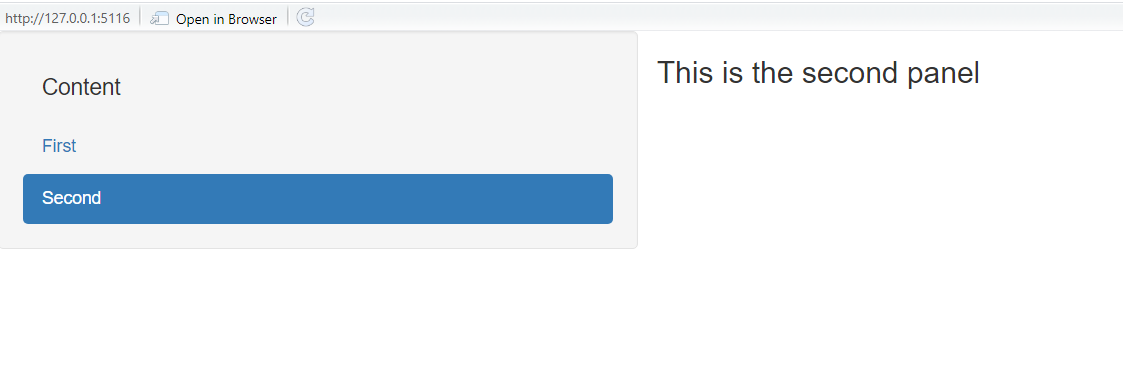
\includegraphics[width=1\textwidth]{figure/navlistPanel.png}
  \end{figure}
\end{frame}



\begin{frame}[fragile]{1. Ebene: Navigation II}
  \begin{itemize}
    \item \href{https://shiny.rstudio.com/gallery/navbar-example.html}{\underline{navbarPage()}}: Navigationsliste für einzelne Seiten ($\rightarrow tabPanel()$) oben
  \end{itemize}
\begin{knitrout}\small
\definecolor{shadecolor}{rgb}{0.969, 0.969, 0.969}\color{fgcolor}\begin{kframe}
\begin{alltt}
\hlcom{#ui.r:}
\hlkwd{navbarPage}\hlstd{(}\hlstr{"Content"}\hlstd{,}
  \hlkwd{tabPanel}\hlstd{(}\hlstr{"First"}\hlstd{,} \hlkwd{h3}\hlstd{(}\hlstr{"This is the first panel"}\hlstd{)),}
  \hlkwd{navbarMenu}\hlstd{(}\hlstr{"More"}\hlstd{,}
    \hlkwd{tabPanel}\hlstd{(}\hlstr{"Second"}\hlstd{,} \hlkwd{h3}\hlstd{(}\hlstr{"This is the second panel"}\hlstd{)),}
    \hlkwd{tabPanel}\hlstd{(}\hlstr{"Third"}\hlstd{,} \hlkwd{h3}\hlstd{(}\hlstr{"This is the third panel"}\hlstd{))}
  \hlstd{)}
\hlstd{)}
\end{alltt}
\end{kframe}
\end{knitrout}
  \begin{figure}
  	\centering
  	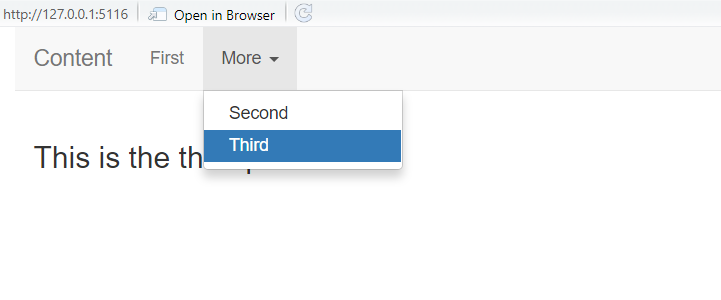
\includegraphics[width=1\textwidth]{figure/navbarPage.png}
  \end{figure}
\end{frame}  



\begin{frame}[fragile]{2. Ebene: Aufteilung der Seite}
  \begin{itemize}
     \item \href{https://www.bioinformatics.babraham.ac.uk/shiny/Intro_to_Shiny_course/examples/04.1_layouts/}{\underline{sidebarLayout()}}: Aufteilung der Seite zwei Spalten
  \end{itemize}
\begin{knitrout}\small
\definecolor{shadecolor}{rgb}{0.969, 0.969, 0.969}\color{fgcolor}\begin{kframe}
\begin{alltt}
\hlcom{#ui.r:}
\hlkwd{sidebarLayout}\hlstd{(}
  \hlkwd{sidebarPanel}\hlstd{(}
    \hlkwd{h3}\hlstd{(}\hlstr{"This is the sidebar"}\hlstd{)}
  \hlstd{),}
  \hlkwd{mainPanel}\hlstd{(}
    \hlkwd{h3}\hlstd{(}\hlstr{"This is the main panel"}\hlstd{)}
  \hlstd{)}
\hlstd{)}
\end{alltt}
\end{kframe}
\end{knitrout}
  \begin{figure}
  	\centering
  	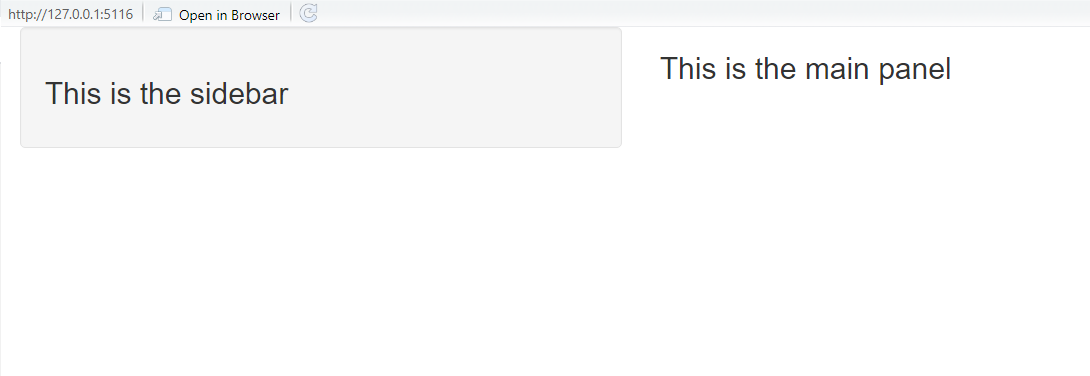
\includegraphics[width=1\textwidth]{figure/sidebarLayout.png}
  \end{figure}  
\end{frame}


\begin{frame}[fragile]{3. Ebene: Tab-Struktur auf einer Seite}
  \begin{itemize}
     \item \href{https://shiny.rstudio.com/gallery/tabsets.html}{\underline{tabsetPanel()}}: Box die verschiedene Tabs darstellen kann 
  \end{itemize}
\begin{knitrout}\small
\definecolor{shadecolor}{rgb}{0.969, 0.969, 0.969}\color{fgcolor}\begin{kframe}
\begin{alltt}
\hlcom{#ui.r:}
\hlkwd{tabsetPanel}\hlstd{(}\hlkwc{type} \hlstd{=} \hlstr{"tabs"}\hlstd{,}
            \hlkwd{tabPanel}\hlstd{(}\hlstr{"First"}\hlstd{,}
                     \hlkwd{h3}\hlstd{(}\hlstr{"This is the first tab"}\hlstd{)),}
            \hlkwd{tabPanel}\hlstd{(}\hlstr{"Second"}\hlstd{,}
                     \hlkwd{h3}\hlstd{(}\hlstr{"This is the second tab"}\hlstd{)),}
            \hlkwd{tabPanel}\hlstd{(}\hlstr{"Third"}\hlstd{,}
                     \hlkwd{h3}\hlstd{(}\hlstr{"This is the third tab"}\hlstd{))}
\hlstd{)}
\end{alltt}
\end{kframe}
\end{knitrout}
  \begin{figure}
  	\centering
  	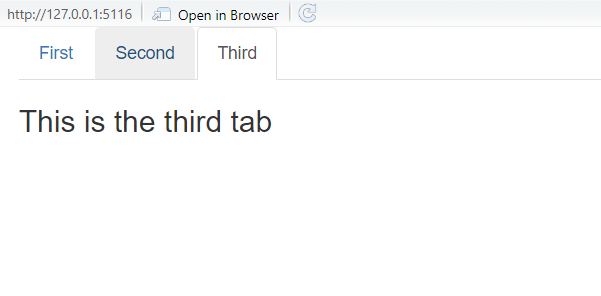
\includegraphics[width=1\textwidth]{figure/tabsetPanel.png}
  \end{figure}    
\end{frame}


        
\begin{frame}[fragile]{4. Ebene: Platzierung der Elemente auf Seite}        
  \begin{itemize}
    \item fluidRow(): Alle Elemente innerhalb, werden in einer Zeile dargestellt
    \item column(): Definiert die Spalten innerhalb der Zeile
  \end{itemize} 
\begin{knitrout}\small
\definecolor{shadecolor}{rgb}{0.969, 0.969, 0.969}\color{fgcolor}\begin{kframe}
\begin{alltt}
\hlcom{#ui.r:}
\hlkwd{fluidRow}(\hlkwd{column}(2, \hlkwd{h3}(\hlstr{"row:1 / column: 1"})),
         \hlkwd{column}(2, \hlkwd{h3}(\hlstr{"row:1 / column: 2"})),
         \hlkwd{column}(2, \hlkwd{h3}(\hlstr{"row:1 / column: 3"}))
),
\hlkwd{fluidRow}(\hlkwd{column}(1, \hlkwd{h3}(\hlstr{"row:2 / column: 1"})),
         \hlkwd{column}(1, \hlkwd{h3}(\hlstr{"row:2 / column: 2"})),
         \hlkwd{column}(1, \hlkwd{h3}(\hlstr{"row:2 / column: 3"}))
)
\end{alltt}
\end{kframe}
\end{knitrout}
  \begin{figure}
  	\centering
  	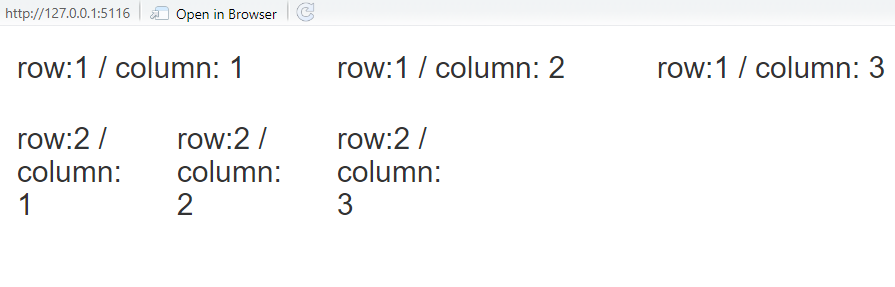
\includegraphics[width=1\textwidth]{figure/fluidRowandcolumn.png}
  \end{figure}  
\end{frame}



\begin{frame}{Darstellung des Inhalts}        
  \begin{itemize}
    \item In Shiny können vereinfacht HTML-Befehlte genutzt werden, um Inhalte in bestimmter Form darzustellen
  \end{itemize}
  
  \begin{table}[]
  \begin{tabular}{lll}
  \hline \hline
  \textbf{Shiny} & \textbf{HTML}                                           & \textbf{Content}          \\ \hline
  p()            & \textless{}p\textgreater{}                              & A paragraph of text       \\
  h1() - h6()    & \textless{}h1\textgreater - \textless{}h6\textgreater{} & Header of different level \\
  a()            & \textless{}a\textgreater{}                              & Hyperlink                 \\
  img()          & \textless{}img\textgreater{}                            & Image                     \\
  br()           & \textless{}br\textgreater{}                             & Line break                \\
  strong()       & \textless{}strong\textgreater{}                         & Bold text                 \\
  em()           & \textless{}em\textgreater{}                             & Italicized text           \\
  HTML()         &                                                         & Directly pass HTML code   \\ \hline \hline
  \end{tabular}
  \end{table} 
\end{frame}


\begin{frame}{}
  \centering
  \textbf{Übung in R: '1 Structure'}
\end{frame}





%--------------------------------------------------------------%
%---------------------- Inputs: Widgets -----------------------%
%--------------------------------------------------------------%

\section{Inputs: Widgets} % important for content page


\begin{frame}{Widgets}
    \begin{itemize}
      \item Widgets sind interaktive Webelemente
      \item Diese erfüllen insbesondere die Funktion Input von Usern entgegen zu nehmen
      \item Das Shiny-Packet beinhaltet eine Reihe von \href{https://shiny.rstudio.com/gallery/widget-gallery.html}{\underline{Build-in Widgets}}
      \item Das Paket \href{http://shinyapps.dreamrs.fr/shinyWidgets/}{\underline{shinyWidgets}} stellt weitere Widgets zur Verfügung
    \end{itemize}
    
  \begin{figure}
  	\centering
  	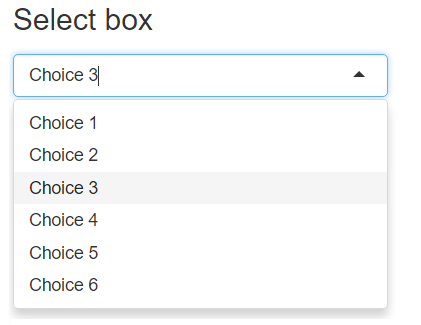
\includegraphics[width=0.4\textwidth]{figure/SelectBox-Widget.png}
  \end{figure}

\end{frame}


\begin{frame}[fragile]{Nutzung von Widgets}
    \begin{itemize}
      \item Widgets werden in der ui.r definiert
      \item Benötigen verschiedene Inputs für Argumente 
        \begin{itemize}
        \item check $help(<command>)$
        \end{itemize}
      \item Erstes Argument ist meist die 'inputId' des Widgets
      \item Mittels der \textbf{'inputId'} kann der Input des Widgets (z.B. eine Zahl) im \underline{Server} abgerufen werden 
    \end{itemize}
\begin{knitrout}\small
\definecolor{shadecolor}{rgb}{0.969, 0.969, 0.969}\color{fgcolor}\begin{kframe}
\begin{alltt}
\hlcom{#ui.r:}
\hlkwd{fluidPage}\hlstd{(}
    \hlcom{# Application title}
      \hlkwd{titlePanel}\hlstd{(}\hlstr{"My first App"}\hlstd{),}
    \hlcom{#Numeric input}
      \hlkwd{numericInput}\hlstd{(}\hlstr{"num"}\hlstd{,} \hlkwc{label} \hlstd{=} \hlkwd{h3}\hlstd{(}\hlstr{"Numeric input"}\hlstd{),}
                   \hlkwc{value} \hlstd{=} \hlnum{1}\hlstd{),}
    \hlcom{#Text input}
      \hlkwd{textInput}\hlstd{(}\hlstr{"text"}\hlstd{,} \hlkwc{label} \hlstd{=} \hlkwd{h3}\hlstd{(}\hlstr{"Text input"}\hlstd{),}
                \hlkwc{value} \hlstd{=} \hlstr{"Enter text..."}\hlstd{),}
    \hlstd{...}
\hlstd{)}
\end{alltt}
\end{kframe}
\end{knitrout}
\end{frame}


\begin{frame}{}
  \centering
  \textbf{Übung in R: '2 Widgets'}
\end{frame}





%------------------------------------------------------%
%---------------------- Outputs -----------------------%
%------------------------------------------------------%

\section{Outputs} % important for content page

\begin{frame}[fragile]{Outputs}
  \begin{itemize}
    \item In server.r \& ui.r werden Änderungen vorgenommen 
    \item server: Hier wird der Output erstellt und "gerendert"
      \begin{itemize}
        \item Output-Erstellung: z.B Produktion einer Grafik mittels ggplot()
        \item Rendering: Transformation des R-Outputs in eine von Browsern lesbare Sprache (JS, HTML, CSS, o.ä.)
      \end{itemize}
    \item ui: Hier wird ein Platzhalter für den Output benötigt (passend zum render***-Befehl im Server)
  \end{itemize}
  
  \begin{table}[]
  \small
  \begin{tabular}{lll}
  \hline \hline
  \multicolumn{1}{c}{\textbf{\begin{tabular}[c]{@{}c@{}}Server\\ (Render function)\end{tabular}}} & \multicolumn{1}{c}{\textbf{\begin{tabular}[c]{@{}c@{}}User Interface\\ (Output function)\end{tabular}}} & \multicolumn{1}{c}{\textbf{Content}}                                                         \\ \hline
  renderDataTable(\{\})                                                                           & dataTableOutput()                                                                                       & DataTable                                                                                    \\
  renderPlot(\{\})                                                                                & plotOutput()                                                                                            & Plots                                                                                        \\
  renderTable(\{\})                                                                               & tableOutput()                                                                                           & \begin{tabular}[c]{@{}l@{}}data frame, matrix,\\ other table \\ like structures\end{tabular} \\
  renderImage(\{\})                                                                               & imageOutput()                                                                                           & images                                                                                       \\
  renderText(\{\})                                                                                & textOutput()                                                                                            & character strings                                                                            \\ \hline \hline
  \end{tabular}
  \end{table}
  
\end{frame}  
  
  
  
\begin{frame}[fragile]{1 Schritt: Platzhalter setzen in ui.r & server.r}  
\begin{knitrout}\small
\definecolor{shadecolor}{rgb}{0.969, 0.969, 0.969}\color{fgcolor}\begin{kframe}
\begin{alltt}
\hlcom{#ui.r:}
\hlkwd{fluidPage}(
\hlcom{    # Application title}
      \hlkwd{titlePanel}(\hlstr{"My first App"}),
\hlcom{    #Slider Bar}
      \hlkwd{sliderInput}(\hlstr{"obs"}, \hlstr{"Number of observations:"}, 
                  min = 1, max = 50, value = 5)
\hlcom{    #Histogram-Output  }
      \hlkwd{plotOutput}(\hlstr{"histPlot"}), # <- NEW
)
\end{alltt}
\end{kframe}
\end{knitrout}


\begin{knitrout}\small
\definecolor{shadecolor}{rgb}{0.969, 0.969, 0.969}\color{fgcolor}\begin{kframe}
\begin{alltt}
\hlcom{#server.r:}
\hlkwd{shinyServer}\hlstd{(}\hlkwa{function}\hlstd{(}\hlkwc{input}\hlstd{,} \hlkwc{output}\hlstd{) \{}
  \hlcom{#Histogram-Creation}
    \hlstd{output}\hlopt{$}\hlstd{histPlot} \hlkwb{<-} \hlkwd{renderPlot}\hlstd{(\{} \hlcom{# <- NEW}
    \hlstd{\})}
\hlstd{\})}
\end{alltt}
\end{kframe}
\end{knitrout}
\end{frame}


\begin{frame}[fragile]{2 Schritt: Server-Code ausbauen}  
  \begin{itemize}
    \item Einsetzen des eigentliches R-Codes zur Erstellung des Histograms
    \item Hier wird ein Histogramm erzeugt, dass die Werte der Variable $'speed'$ des $'cars'$ Datensatzes darstellt
  \end{itemize}

\begin{knitrout}\small
\definecolor{shadecolor}{rgb}{0.969, 0.969, 0.969}\color{fgcolor}\begin{kframe}
\begin{alltt}
\hlcom{#server.r:}
\hlkwd{shinyServer}\hlstd{(}\hlkwa{function}\hlstd{(}\hlkwc{input}\hlstd{,} \hlkwc{output}\hlstd{) \{}
  \hlcom{#Histogram-Creation}
    \hlstd{output}\hlopt{$}\hlstd{histPlot} \hlkwb{<-} \hlkwd{renderPlot}\hlstd{(\{}
      \hlkwd{hist}\hlstd{(cars}\hlopt{$}\hlstd{speed)}
    \hlstd{\})}
\hlstd{\})}
\end{alltt}
\end{kframe}
\end{knitrout}
\end{frame}


\begin{frame}{}
  \centering
  \textbf{Übung in R: '3 Outputs'}
\end{frame}


%---------------------------------------------------------%
%---------------------- Reactivity -----------------------%
%---------------------------------------------------------%

\section{Reactivity} % important for content page

\begin{frame}[fragile]{Reactivity: Overview} 
\begin{itemize}
  \item Drei Arten von $reaktive objects$ in Shiny:
    \begin{itemize}
      \item Reactive \underline{sources}: Ist in der Regel eine Benutzereingabe über eine Browser-Oberfläche (Widgets: $input\$*$)
      \item Reactive \underline{conductors}: Komponente zwischen source \& endpoint. Kapselung rechenintensiver o. wiederholter Operationen 
      \item Reactive \underline{endpoints}: Normalerweise etwas, das im Browserfenster des Benutzers angezeigt wird ($output\$*$)
    \end{itemize}
  \item Reactive conductors \& endpoints werden erneut ausgeführt, wenn sich min. eine beinhaltete source ändert
  \item Reactive endpoints werden erneut ausgeführt, wenn sich min. ein(e) beinhaltete source o. conductor ändert
  \end{itemize}  
\end{frame}



\begin{frame}{Reactivity: Konzepte \& Umsetzung in R-Shiny} 
  \begin{table}[]
  \begin{tabular}{ccl}
  \hline \hline
  \textbf{\begin{tabular}[c]{@{}c@{}}Allg.\\ Konzepte\end{tabular}} & \textbf{\begin{tabular}[c]{@{}c@{}}Umsetzung\\ in R Shiny\end{tabular}} & \multicolumn{1}{c}{\textbf{Eigenschaften}}                                                                                                               \\ \hline
  \begin{tabular}[c]{@{}c@{}}Reactive \\ source\end{tabular}        & \begin{tabular}[c]{@{}c@{}}reactive \\ value\end{tabular}               & \begin{tabular}[c]{@{}l@{}}- Reagieren auf User-Inputs\\ - Geben einen Wert aus\end{tabular}                                                             \\ \hline
  \begin{tabular}[c]{@{}c@{}}Reactive \\ conductor\end{tabular}     & \begin{tabular}[c]{@{}c@{}}reactive \\ expression\end{tabular}          & \begin{tabular}[c]{@{}l@{}}- Reagieren auf $reactive~values$ \& \\ andere $reactive~expressions$\\ - Geben einen Wert aus\end{tabular}                   \\ \hline
  \begin{tabular}[c]{@{}c@{}}Reactive \\ endpoint\end{tabular}      & observer                                                                & \begin{tabular}[c]{@{}l@{}}- Reagieren auf $reactive~values$ \& \\ $reactive~expressions$\\ - Geben keinen Wert aus \\ - Haben side effects\end{tabular} \\ \hline \hline
  \end{tabular}
  \end{table}
\end{frame}



\begin{frame}[fragile]{Reactivity: Commands}  
  \begin{itemize}
  \item Reactive \underline{values}:
    \begin{itemize}
      \item \textbf{*Input({})}: Evaluiert Code immer wieder, wenn sich einer der beinhalteten reaktive values ändert
      \item \textbf{reactiveValues()}: Definiert ein R-Objekt als Speicherplatz für reactive values
    \end{itemize}  
  \item Reactive \underline{expressions}:
    \begin{itemize}
      \item \textbf{reactive({})}: Erstellt eine $reactive~expression$  
    \end{itemize}
  \item \underline{Observer}:
    \begin{itemize}
      \item \textbf{render*({})}: Erzeugt einen observer output\$*. Wird bei veränderten zugehörigen $reactive~values$ \& $reactive~expressions$ erneut ausgeführt
      \item \textbf{observeEvent(eventExpr, Expr)}: Ausführung des beinhaleteten Codes, nur wenn sich $<eventExpr>$ ändert
      \item \textbf{observe()}: Wie reactive(), nur das keine Ausgabe erzeugt wird
    \end{itemize}
  \item Others:
    \begin{itemize}
      \item isolate(): Unterrückt die Reaktivität eines R-Objekts
    \end{itemize}
 \end{itemize}
\end{frame}


\begin{frame}[fragile]{2 Schritt: Server-Code (reaktiv) ausbauen}  
  \begin{itemize}
    \item Einsetzen des eigentliches R-Codes zur Erstellung des Histograms
    \item Das Histogramm reagiert auf den Input mittels 'input\$obs'
      \begin{itemize}
        \item Hiermit wird der Wert des sliderInputs abgerufen
        \item Der Datensatz wird auf die jeweilige Fallzahl beschränkt
      \end{itemize}
    \item render*()-Funktionen aktualisieren sich automatisch sobald sich der Wert eines enthaltenen Inputs ($\rightarrow input\$*$) ändert
  \end{itemize}

\begin{knitrout}\small
\definecolor{shadecolor}{rgb}{0.969, 0.969, 0.969}\color{fgcolor}\begin{kframe}
\begin{alltt}
\hlcom{#server.r:}
\hlkwd{shinyServer}\hlstd{(}\hlkwa{function}\hlstd{(}\hlkwc{input}\hlstd{,} \hlkwc{output}\hlstd{) \{}
  \hlcom{#Histogram-Creation}
    \hlstd{output}\hlopt{$}\hlstd{histPlot} \hlkwb{<-} \hlkwd{renderPlot}\hlstd{(\{}
      \hlstd{data} \hlkwb{<-} \hlstd{cars}\hlopt{$}\hlstd{speed[}\hlnum{1}\hlopt{:}\hlstd{input}\hlopt{$}\hlstd{obs]}
      \hlkwd{hist}\hlstd{(data)}
    \hlstd{\})}
\hlstd{\})}
\end{alltt}
\end{kframe}
\end{knitrout}
\end{frame}


\begin{frame}{Reactivity: Reactive Graph}  
  \begin{figure}
  	\centering
  	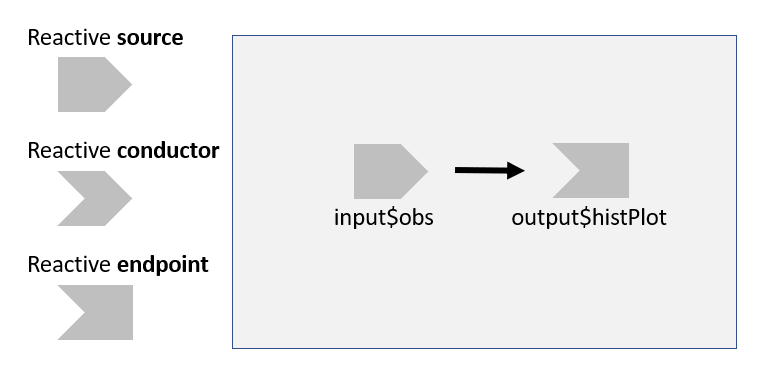
\includegraphics[width=1\textwidth]{figure/ReactiveGraph.png}
  \end{figure}
\end{frame}


\begin{frame}{}
  \centering
  \textbf{Übung in R: '4 Reactivity'}
\end{frame}


%-------------------------------------------------------------%
%----------------- Besprechung & Ausblick --------------------%
%-------------------------------------------------------------%

\section{Besprechung \& Ausblick} % Wichtig für Inhaltsverzeichnis


\begin{frame}{Ausblick} 
  \begin{itemize}
    \item Dashboards mit Shiny:
    \begin{itemize}
      \item \href{http://rstudio.github.io/shinydashboard/get_started.html}{\underline{shinydashboard}}: UI mit Shiny code
       \item \href{https://rmarkdown.rstudio.com/flexdashboard/}{\underline{flexdashboard}}: UI mit R Markdown
     \end{itemize}
  \end{itemize}
  
  \begin{figure}
    	\centering
    	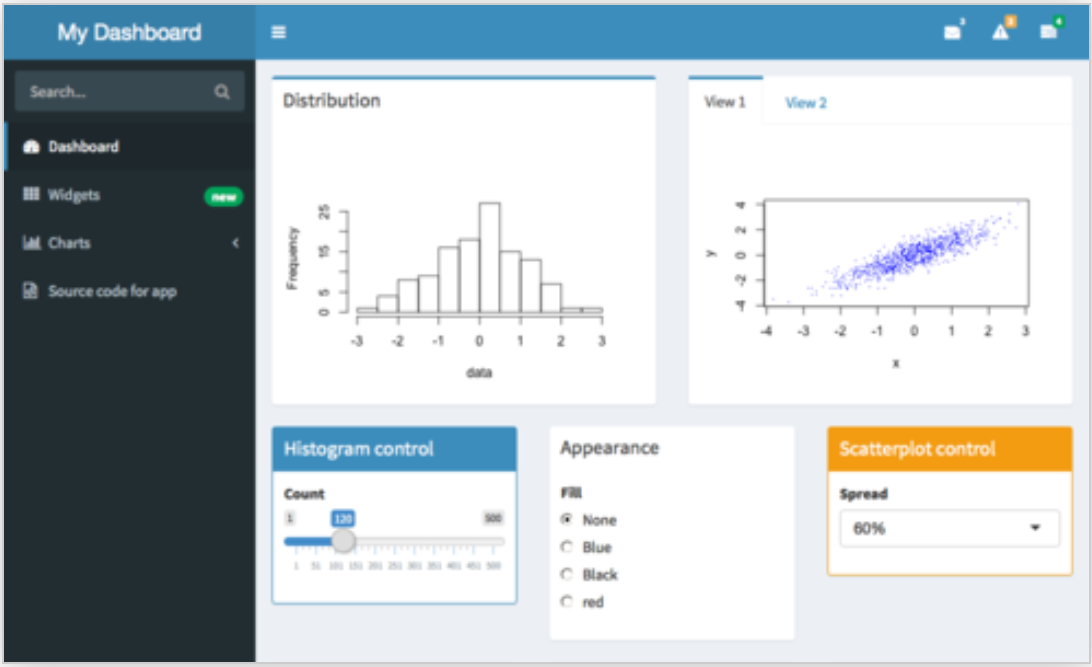
\includegraphics[width=0.5\textwidth]{figure/shinydashboard-example.png}
    \end{figure}  
    
  \begin{itemize}
    \item Komplexere reaktive Verpflechtungen
    \item Öffnung, Veränderung \& Speicherung von Datensätzen
    \item Interaktive web-basierte Datenvisualisierung: \href{https://plotly-r.com/}{\underline{plotly}}
  \end{itemize}
\end{frame}



\begin{frame}{Literatur}
  \begin{itemize}
    \item \href{https://shiny.rstudio.com/}{R-Shiny Homepage}
    \item \href{https://rstudio.github.io/shinythemes/}{Shiny Themes}
    \item \href{https://rstudio.github.io/shiny/tutorial}{Shiny tutorial}
    \item \href{https://shiny.rstudio.com/articles/layout-guide.html}{Shiny Layout guide}
    \item \href{https://shiny.rstudio.com/gallery/widget-gallery.html}{Shiny Build-in Widgets}
    \item \href{https://shiny.rstudio.com/reference/shiny/}{Shiny Function reference}
    \item \href{https://shiny.rstudio.com/gallery/}{Huge collection of exemplary Shiny Apps}
    \item \href{http://rstudio.github.io/shinydashboard/get_started.html}{shinydashboard}
  \end{itemize}
\end{frame}  
  

%Noch Fragen
\begin{frame}

\center{Gibt es noch weitere Fragen?}
  
\end{frame} 


\end{document}
